\documentclass[11pt,a4paper,oneside]{book}
%\usepackage[utf8]{inputenc} 	
\usepackage{a4wide}                     % Iets meer tekst op een bladzijde
\usepackage[english,dutch]{babel}               % Voor nederlandstalige hyphenatie (woordsplitsing)
\usepackage{amsmath}                    % Uitgebreide wiskundige mogelijkheden
\usepackage{amssymb}                    % Voor speciale symbolen zoals de verzameling Z, R...
\usepackage{makeidx}                    % Om een index te maken
\usepackage{url}                        % Om url's te verwerken
\usepackage{graphicx}                   % Om figuren te kunnen verwerken
\usepackage[small,bf,hang]{caption}     % Om de captions wat te verbeteren
\usepackage{xspace}                     % Magische spaties na een commando
\usepackage[latin1]{inputenc}           % Om niet ascii karakters rechtstreeks te kunnen typen
\usepackage{float}                      % Om nieuwe float environments aan te maken. Ook optie H!
\usepackage{flafter}                    % Opdat floats niet zouden voorsteken
\usepackage{listings}                   % Voor het weergeven van letterlijke text en codelistings
\usepackage[round]{natbib}              % Voor auteur-jaar citaties.
\usepackage[nottoc]{tocbibind}		% Bibliografie en inhoudsopgave in ToC; zie tocbibind.dvi
\usepackage{eurosym}                    % om het euro symbool te krijgen
\usepackage{textcomp}                   % Voor onder andere graden celsius
\usepackage{fancyhdr}                   % Voor fancy headers en footers
\usepackage[Gray,squaren,thinqspace,thinspace]{SIunits} % Om elegant eenheden te zetten
\usepackage[version=3]{mhchem}          % Voor elegante scheikundige formules
\usepackage{pdfpages}					% Pdf includeren
\usepackage{subcaption}					% 2 figuren naast mekaar, met elk een caption
\usepackage[bottom]{footmisc}			% footnotes forceren naar bottom
\usepackage{nomencl}					%afkortingen
\makenomenclature %update bij every run
\renewcommand{\nomname}{Lijst van afkortingen}

% Volgend package is niet echt nodig. Het laat echter toe om gemakkelijk elektronisch
% te navigeren in je pdf-document. Deze package moet altijd als laatste ingeladen worden.
\usepackage[a4paper,plainpages=false]{hyperref}    % Om hyperlinks te hebben in het pdfdocument.


%%%%%%%%%%%%%%%%%%%%%%%%%%%%%%
% Algemene instellingen van het document.
%%%%%%%%%%%%%%%%%%%%%%%%%%%%%%

% De splitsingsuitzonderingen
\hyphenation{back-slash split-sings-uit-zon-de-ring}

%\bibpunct{(}{)}{;}{y}{,}{,}             % Auteur-jaar citaties -- zie natbib.dvi voor meer uitleg; niet echt nodig

% Het bibliografisch opmaak bestand.
% ZORG ERVOOR DAT bibliodutch.bst ZICH IN JE WERKDIRECTORY BEVINDT!!!
\bibliographystyle{bibliodutch}

\setlength{\parindent}{0cm}             % Inspringen van eerste lijn van paragrafen is niet gewenst.

\renewcommand{\baselinestretch}{1.2} 	% De interlinie afstand wat vergroten.

\graphicspath{{figuren/}}               % De plaars waar latex zijn figuren gaat halen.

\makeindex                              % Om een index te genereren.

\setcounter{MaxMatrixCols}{20}          % Max 20 kolommen in een matrix

% De headers die verschijnen bovenaan de bladzijden, herdefinieren:
\pagestyle{fancy}                       % Om aan te geven welke bladzijde stijl we gebruiken.
\fancyhf{}                              % Resetten van al de fancy settings.
\renewcommand{\headrulewidth}{0pt}      % Geen lijn onder de header. Zet dit op 0.4pt voor een mooie lijn.
\fancyhf[HL]{\nouppercase{\textit{\leftmark}}} % Links in de header zetten we de leftmark,
\fancyhead[HR]{\thepage}                % Rechts in de header het paginanummer.
% Activeer de volgende lijn en desactiveer de vorige om paginanummers onderaan gecentreerd te krijgen.
%\fancyhf[FC]{\thepage}                  % Paginanummers onderaan gecentreerd.

% PDF specifieke opties, niet strict noodzakelijk voor een thesis.
% Is hetgeen verschijnt wanneer je in acroread de documentproperties bekijkt.
\hypersetup{
    pdfauthor = {Andreas De Lille},
    pdftitle = {Automatische testbed monitoring voor toekomstig internetonderzoek},
    pdfsubject = {Scriptie van de masterproef Automatische testbedmonitoring voor toekomstig internet onderzoek},
    pdfkeywords = {testbed, jFed, monitoring, webservice, eindwerk, scriptie}
}


% Het volgende commando zou ervoor moeten zorgen dat er een witte ruimte wordt gelaten tussen
% elke paragraaf. Het zorgt ervoor dat er echter teveel witte ruimte komt boven en onder de
% verschillende titels, gemaakt met \section, subsection...
%%\setlength{\parskip}{0ex plus 0.3ex minus 0.3ex}

% Vandaar dat we expliciet aangeven wanneer we wensen dat een nieuwe paragraaf begint:
% \par zorgt ervoor dat er een nieuwe paragraaf begint en
% \vspace zorgt voor vertikale ruimte.
\newcommand{\npar}{\par \vspace{2.3ex plus 0.3ex minus 0.3ex}}

%%%%%%%%%%%%%%%%%%%%%%%%%%%%%%
% Nieuwe commando's
%%%%%%%%%%%%%%%%%%%%%%%%%%%%%%

% De differentiaal operator
\newcommand{\diff}{\ensuremath{\mathrm{d}}} 

% Super en subscript
\newcommand{\supsc}[1]{\ensuremath{^{\text{#1}}}}   % Superscript in tekst
\newcommand{\subsc}[1]{\ensuremath{_{\text{#1}}}}   % Subscript in tekst

% Chemische formule font:
\newcommand{\ch}[1]{\ensuremath{\mathrm{#1}}\xspace}	 
% Chemische pijl naar rechts:
\newcommand{\chpijlr}{\ensuremath{\hspace{1em}\longrightarrow\hspace{1em}}}
% Chemische pijl naar links:
\newcommand{\chpijll}{\ensuremath{\hspace{1em}\longleftarrow\hspace{1em}}}
% Chemische pijl naar links en rechts:
\newcommand{\chpijllr}{\ensuremath{\hspace{1em}\longleftrightarrow\hspace{1em}}}

\newcommand{\vt}[1]{\ensuremath{\boldsymbol{#1}}} % vector in juiste lettertype
\newcommand{\mx}[1]{\ensuremath{\mathsf{#1}}}	  % matrix in juiste lettertype

% Het latex logo in een eenvoudiger commando steken
\newcommand{\latex}{\LaTeX\xspace}

% Het BibTeX logo
\newcommand{\bibtex}{\textsc{Bib}\TeX\xspace}

% Niew commando om bestandnamen anders weer te geven
\newcommand{\bestand}[1]{\lstinline[basicstyle=\sl]{#1}\xspace}

% Niew commando om commando tekst weer te geven
\newcommand{\command}[1]{\lstinline[basicstyle=\tt]{#1}\xspace}
\newcommand{\commandx}[1]{\index{#1}\lstinline[basicstyle=\tt]{#1}\xspace}

%\lstset{morecomment={\%}}
% Commando om latex commando`s weer te geven (x: voor indexing)
%\newcommand{\lcommand}[1]{\lstinline[basicstyle={\tt},{language=[LaTeX]TeX}]{#1}\xspace}
\newcommand{\lcommand}[1]{\lstinline[basicstyle={\tt}]{#1}\xspace}
\newcommand{\lcommandx}[1]{\index{#1}\lstinline[basicstyle=\tt]{#1}\xspace}


% Niew commando om vreemde taal weer te geven (hint: dit commando kan gebruikt
%   worden om latijnse namen, die ook cursief moeten staan, weer te geven.
\newcommand{\engels}[1]{\textit{#1}\xspace}
\newcommand{\engelsx}[1]{\index{#1}\textit{#1}\xspace}

% Niew commando om iets te benadrukken en tegelijkertijd in de index te steken.
\newcommand{\begrip}[1]{\index{#1}\textbf{#1}\xspace}

% Nieuw commando om figuren in te voegen. Gebruik:
% \mijnfiguur[H]{width=5cm}{bestandsnaam}{Het bijschrift bij deze figuur}
\newcommand{\mijnfiguur}[4][H]{            % Het eerste argument is standaar `ht'. op H zetten voor HIER EN NERGENS ANDERS
    \begin{figure}[#1]                      % Beginnen van de figure omgeving
        \begin{center}                      % Beginnen van de center omgeving
            \includegraphics[#2]{#3}        % Het eigenlijk invoegen van de figuur (2: opties, 3: bestandsnaam)
            \caption{#4\label{#3}}          % Het bijschrift (argument 4) en het label (argument 3)
        \end{center}
    \end{figure}
    }
		
% Nieuw commando om figuren in te voegen. Gebruik:
% \mijnfiguur[H]{bestand-tabular}{Het bijschrift bij deze tabel}    
\newcommand{\mijntabel}[3][ht]{             % Het eerste argument is standaar `ht'.
    \begin{table}[#1]                       % Beginnen van de table omgeving
        \begin{center}                      % Beginnen van de center omgeving
            \caption{#3\label{#2}}          % Het bijschrift (argument 3) en het label (argument 2)
            \input{#2}                      % Invoer van de tabel
        \end{center}
    \end{table}
}

%quoten
\newcommand{\quotes}[1]{\lq #1\rq\xspace}

%%%%%%%%%%%%%%%%%%%%%%%%%%%%%%
% Nieuwe wiskunde operatoren
%%%%%%%%%%%%%%%%%%%%%%%%%%%%%%

\DeclareMathOperator{\integ}{Integraal}

%%%%%%%%%%%%%%%%%%%%%%%%%%%%%%
% Nieuwe omgevingen
%%%%%%%%%%%%%%%%%%%%%%%%%%%%%%

% Een soort theorem omgeving
\newtheorem{levensles}{Levensles}[chapter]

% Om minder belangrijke delen iets kleiner te zetten.
\newenvironment{MinderBelangrijk}{\small}{}

% Een nieuwe omgeving om letterlijke latex tekst weer te geven.
\lstnewenvironment{llt} 
    {
    \vspace{1.2ex plus 0.5ex minus 0.5ex}   % Beetje ruimte voor de letterlijke tekst
    \lstset{                                % Enkele opties:
        basicstyle={\small\tt},             % Iets kleiner
        %language=[LaTeX]{TeX},              % Syntax highlighting
        stepnumber=0,                       % De lijnen worden niet genummerd
        breaklines=true,                    % Als een lijn te lang is, wordt hij afgebroken
        basewidth={0.5em},                  % Breedte van een letter
        xleftmargin=1em}                    % Inspringing van de linker marge
    }
    {\vspace{0.9ex plus 0.5ex minus 0.5ex}  % Beetje ruimte na de letterlijke tekst
    }

% Een nieuwe omgeving om algemene letterlijke tekst weer te geven.
\lstnewenvironment{lt} 
    {
    \vspace{1.2ex plus 0.5ex minus 0.5ex}   % Beetje ruimte voor de letterlijke tekst
    \lstset{                                % Enkele opties:
        basicstyle={\small\tt},             % Iets kleiner en typmachine lettertype
        stepnumber=0,                       % De lijnen worden niet genummerd
        breaklines=true,                    % Als een lijn te lang is, wordt hij afgebroken
        basewidth={0.5em},                  % Breedte van een letter
        xleftmargin=1em}                    % Inspringing van de linker marge
    }
    {\vspace{0.9ex plus 0.5ex minus 0.5ex}  % Beetje ruimte na de letterlijke tekst
    }

\newenvironment{samenvatting}{\small\itshape}{}

\lstset{
	language={Python},
	showspaces=false,
	showstringspaces=false
}

%%%%%%%%%%%%%%%%%%%%%%%%%%%%%%
% Einde van de preamble.
% Begin van de body:
%%%%%%%%%%%%%%%%%%%%%%%%%%%%%%

\begin{document}

\frontmatter


\includepdf[pages={1}]{titelblad.pdf}       %titelblad

%
% Typisch copyright voor een thesis.
% Te plaatsen juist na het titelblad.

\rule[-0.4\baselineskip]{0cm}{10\baselineskip}   
\par \vspace{2.3ex plus 0.3ex minus 0.3ex}
De auteur en promotor geven de toelating deze scriptie voor consultatie beschikbaar te stellen en delen ervan te kopi�ren voor persoonlijk gebruik. Elk ander gebruik valt onder de beperkingen van het auteursrecht, in het bijzonder met betrekking tot de verplichting uitdrukkelijk de bron te vermelden bij het aanhalen van resultaten uit deze scriptie.
\par \vspace{2.3ex plus 0.3ex minus 0.3ex}
The author and promoter give the permission to use this thesis for consultation and to copy parts of it for personal use. Every other use is subject to the copyright laws, more specifically the source must be extensively specified when using from this thesis.
\par \vspace{2.3ex plus 0.3ex minus 0.3ex}
Gent, Juni 2004 % Vul de juiste datum in!!!
\par \vspace{2.3ex plus 0.3ex minus 0.3ex}

De promotor \hfill De begeleider \hfill De auteur
\npar
\vspace{2cm}
\npar
% Pas de volgende lijn aan!!!
Prof. dr. ir. A. Armagneau \hfill Zijnen assistent \hfill Gaspard Lequeux

\thispagestyle{empty} 

                   	% Voor een echte thesis.
%\newpage
%\mbox{}\vspace{-1cm}
%\thispagestyle{plain}

%\textbf{\Huge{Woord vooraf}}

\chapter*{Woord vooraf}

%\vspace{2cm}

\begin{slshape}

%\small
Deze cursus werd in November 2003 voor het eerst uitgegeven in het kader van een Zeus (Studenten Werkgroep Informatica) initiatief om thesistudenten te helpen hun thesis in een aantrekkelijke vorm te gieten. De tekst is opgevat als een soort minithesis zodat studenten gemakkelijk alles kunnen overnemen. Om die reden zijn de bronbestanden beschikbaar gemaakt op het internet.\footnote{\url{http://zeus.ugent.be/~gaspard/latex}} 
\npar
Hoewel sommige deeltjes van deze cursus expliciet gericht zijn op het maken van een thesis, kan de tekst gebruikt worden als algemene inleiding op \latex. In 2004 zag ook Prof. Ottoy dit in. Vandaar dat deze cursus nu deel uitmaakt van de lessen informatica in de tweede bachelor bio-ir van de Universiteit Gent. Bij die gelegenheid heeft hij de cursus volledig nagekeken op taalfouten, waarvoor dank.
\npar
In 2006 heeft Prof. Dawyndt de cursus ook grondig herlezen en nagekeken, waarvoor dank. Sindsdien wordt deze cursus gebruikt in de lessen Computergebruik gegeven in de eerste bachelor Informatica van de Universiteit Gent.
\npar
Voor het schrijven van deze handleiding \latex, werd gebruik gemaakt van twee werken: \textsf{A guide to \latex} van \citet{kopka99} en \textsf{Handleiding \latex} van Piet van Oostrum (1996). Uit dit laatste werden zelfs hele paragrafen overgenomen. Daarnaast werd natuurlijk rijkelijk geput uit de documentatie die meegeleverd wordt met \latex zelf.
\npar
Minder belangrijke delen worden in een kleiner lettertype weergegeven. Verder zijn er verschillende voetnoten die verwijzen naar \latex documentatie op een Debian GNU/Linux systeem. Niemand gebruikt dat natuurlijk. Maar de bedoeling ervan is dat de lezer weet dat de documentatie bestaat, welke bestandsnaam die heeft en waar ongeveer die te vinden is in de \latex directorystructuur. Het is dan niet zo moeilijk meer om in je favoriete besturingssysteem te zoeken naar de desbetreffende bestandsnaam. 
\npar
In een standaard MikTeX installatie (d\'e \latex distributie voor Windows), zijn de helpfiles van de verschillende \latex packages te vinden in \bestand{C:\\texmf\\doc\\latex}. In \bestand{C:\\texmf\\doc\\guides} zijn enkele algemene handleidingen te vinden over \latex.
\npar
Het woord vooraf dient ook om mensen te bedanken: 

\begin{itemize}

\item De mensen van Zeus, voor de stimulerende Vrije--\engels{Open Source} sfeer en het organiseren van lessen hier rond. 

\item Schamper, het studentenblad van de Universiteit Gent, voor het leveren van de promotor van dit werk.

\item Rudy Gevaert, die in het academiejaar 2001-2002 als eerste een \latex les gaf.

\item Geert Vernaeve, voor het eerste contact met \latex en het C-voorbeeld op bladzijde \pageref{cvoorbeeld}.

\item Mensen die fouten rapporteerden en/of verbeteringen suggereerden: David De Wolf, Annelies Huyck, Yves Nevelsteen, Stijn Gors, Geert Vernaeve, Michiel Meire, Hendrik Maryns, Olivier Verhoogen, Jean-Pierre Ottoy, Hugo Coolens, Lieven Clement, Andy Peene, Reinout Debergh, Frederik De Schrijver, David van der Ha, Brecht Donckels, Dominique Lebbe, Christopher De Dobbelaere, Paul Vogels, Heidi Vanparys, Stijn Depuydt, Veerle Gevaert, Joke Van Hevele, Katrien De Dauw, Francis Santens, Nicolas Vanden Bossche en Peter Dawyndt.

\item De (thesis)studenten van het Boerenkot,
%\footnote{Ook nog wel Faculteit Landbouwkundige en Toegepaste Biologische Wetenschappen genoemd, maar niemand gebruikt die lange naam ;-)}
die in 2003 gevraagd hebben naar deze handleiding.

\end{itemize}

\latex lijkt in het begin moeilijk: alles in tekstmode, geen knopjes, je moet speciale commando's kennen om iets te bereiken~\ldots\ De eerste dagen zul je inderdaad enkele problemen ondervinden. Zoeken, doorbijten en hulp vragen aan meer ervaren gebruikers zullen ervoor zorgen dat je na enkele weken zelfs je wiskundige redeneringen rechtstreeks in \latex uitvoert. 
\npar
Deze handleiding is waarschijnlijk niet fautloos. Het rapporteren van meer dan ��n fout, zorgt voor je naam in de volgende editie van dit woord vooraf. Ook inhoudelijke opmerkingen zijn steeds welkom.

\vspace{4ex}

\hfill Gaspard Lequeux

\hfill Gent 9 Augustus 2006

%\normalsize
\end{slshape}

                      	% Algemene versie

% Voor een echte thesis, komt hier de samenvatting...
\newpage
\chapter*{Abstract}
\npar
Door de huidige verschuiving naar cloud-gebaseerde technologi\"en zal het belang 
van netwerkprotocollen en beschikbaarheid van netwerken alleen maar toenemen.
Om deze verschuiving vlot te laten verlopen is er meer en meer onderzoek nodig naar netwerktechnologi\"en.
Voor dit onderzoek wordt er dan ook veelvuldig gebruik gemaakt van testbeds.
Testbeds worden aangestuurd via jFed en worden gebruikt om netwerken te simuleren.
De situatie heeft enkele nadelen. Het is voor een onderzoeker soms erg moeilijk om te bepalen of een bepaald gedrag in hun experiment te wijten is aan de eigen ontwikkelingen, of aan het testbed zelf.
\npar
Deze masterproef zal trachten dit probleem te verhelpen door de testbed monitoring te automatiseren. Via een webservice zal deze informatie dan aangeboden worden. Deze webservice zal weergeven hoe betrouwbaar een testbed is. Hiervoor komen verschillende ontwikkelingstools aan bod. Uiteindelijk zal deze service ervoor zorgen dat een onderzoeker via zijn primaire gebruikersinterface op de hoogte gebracht wordt van eventuele problemen.                            % ...in het Nederlands en...
\newpage
\chapter*{Abstract}
\npar
Due to the new cloud-based technologies, network protocols and network reachability are now more important than ever. To make this change quick and clean, we need more and more network research. FIRE (Future Internet Research and Experimentation) is an European project created to improve the network and internet experimentation. FIRE is the opportunity to jointly develop potentially disruptive innovations for the future of the internet. It is about collaborative research and sharing test facilities. Researchers working for FIRE will now work closer together, sharing ideas. FIRE is also used to share test facilities from all over the world, so researchers have access to many different test facilities.\\

To make handling of these different testbeds easier, jFed was created. jFed is a java tool with the purpose of controlling testbeds. Unfortunately, the current situation has a major downside in that it is very hard for researchers to determine if a certain behavior is caused by the testconfiguration or by the test facility. 
\npar
This thesis will try to solve the aforementioned problem by creating an automated the testbed monitoring system. A monitoringAPI will then share this information. Doing so, will provide future tools easy access to this information.                            % ...in het Engels.
%voorwoord?
%dankwoord?/back	

%afkortingen
\printnomenclature

%figuren
\listoffigures
%tabellen
%\listoftables

% De lijnen van de inhoudsopgave iets dichter op elkaar, niet echt nodig voor de thesis, maar 
% voor dit werk kregen we anders een laatste bladzijde met 3 items op.
\renewcommand{\baselinestretch}{1.08} 	% De interlinie afstand wat vergroten.
\small\normalsize                       % Nodig om de baselinestretch goed te krijgen.
\tableofcontents
\renewcommand{\baselinestretch}{1.2} 	% De interlinie afstand wat vergroten.
\small\normalsize                       % Nodig om de baselinestretch goed te krijgen.
\chapter{Inleiding}
\npar
Het gebruik van netwerken en het internet om computers en allehande randapperatuur te verbinden zal in de toekomst alleen maar stijgen. Het is dan ook van groot belang dat onderzoek op dit gebied vlot en correct verloopt en dat onderzoekers samenwerken om zo idee\"en en nieuwe technologie\"en te delen. Daarnaast moeten er ook testfaciliteiten zijn om deze nieuwe technologie\"en te testen.
FIRE (Future Internet Research and Experimentation) is een Europees onderzoeksprogramma dat zich op deze doelen richt.
\npar
Om de configuratie en de werking van de verschillende testbeds gelijk te maken, is de federation architectuur ontworpen. De invoering hiervan zit in het Fed4FIRE (Federation for FIRE) project. De federation architectuur die in deze masterproef behandeld wordt, is SFA 2.0 (Slice-federation-architecture). Hierbij vormen alle testbeds van FIRE een federatie. Daardoor hebben onderzoekers binnen FIRE toegang tot alle testbeds binnen FIRE.
\npar
Het beheer van al deze verschillende testbeds is geen sinecure. Om dit beheer te vereenvoudigen is er binnen IBCN (Internet Based Communication Networks and Services), een onderdeel van het onderzoekscentrum iMinds, een monitoringsservice gemaakt. Deze service controleert periodiek of de SFA-API nog werkt. Echter door zijn snelle ontwikkeling is de service niet voorzien op uitbreidingen.
\npar
FIRE werkt samen met een gelijkaardig project, GENI. GENI (Global Environment for Network Innovations) is een Amerikaans project met gelijkaardige doelstellingen als FIRE. GENI is ook bezig met de ontwikkeling van een monitoringssysteem dat echter meer de nadruk legt op het monitoren van experimenten. De samenwerking tussen beide projecten kan bevorderd worden als beide monitoringssystemen compatibel zijn.
\npar
De opdracht van deze masterproef bestaat uit 3 grote delen. \\
Het eerste deel is het maken van een API die monitoringsdata beschikbaar maakt voor andere applicaties. Het tweede deel is een monitoringsservice maken die testbeds controleert. Het derde en laatste deel is de monitoringsservice uitbereiden om loadtesten uit te voeren. Met deze loadtesten wordt bekeken welke lading een testbed kan afhandelen.
\clearpage
\npar
De scriptie is al volgt uitgewerkt.
Hoofdstuk 1 Situeert de masterproef. Hier wordt ook kort de opdracht uitgelegd. In hoofdstuk 2 wordt de SFA-architectuur uitgelegd. Deze architectuur wordt gebruikt om de configuratie en besturing van testbeds over heel de wereld gelijk te maken.
\npar
Hoofdstuk 3 geeft meer uitleg over de bestaande FIRE en GENI monitor en geeft hierbij ook de probleemstelling aan. Hoofdstuk 4 geeft bespreekt het ontwerp van de masterproef. In hoofdstuk 5 wordt de implementatie van de verschillende onderdelen besproken.
\npar
Bijlage \ref{REFERENCE} bevat de referentie van de monitoringsAPI, geschreven in Engels.Bijlage \ref{ONDERHOUD}  bevat informatie voor de systeembeheerder.Bijlages \ref{REFERENCE} en \ref{ONDERHOUD} zijn specifiek gericht aan de systeembeheerder en eindgebruikers.

\mainmatter
% De verschillende hoofdstukken:
\chapter{Situering}
{\samenvatting
In dit hoofdstuk wordt het achterliggende kader van de masterproef geschetst. Daarnaast wordt ook de opdracht uitgewerkt. De opdracht bestaat uit 2 grote delen enerzijds een monitoringsservice maken om testbeds te controleren. De informatie van deze monitoringsservice wordt via de monitoringsAPI beschikbaar gesteld aan de buitenwereld. Anderzijds wordt de monitoringsAPI geïntegreerd in een groter Amerikaans framework.}
\section{Situering}
\npar
Deze masterproef is een onderdeel van een groter Europees onderzoeksproject genaamd FIRE (Future Internet Research and Experimentation)\nomenclature{FIRE}{Future Internet Research and Experimentation}. FIRE is gericht is op onderzoek naar toekomstige internet- en netwerktechnologiën. Door onderzoekscentra te laten samenwerken\citep{Fire-what-is}, tracht FIRE het onderzoek vlotter te laten verlopen. FIRE heeft twee grote doelen. Enerzijds de samenwerking tussen verschillende onderzoekscentra te verbeteren, anderzijds het delen van testfacilities makkelijker te maken.
\npar
Het eerste doel is de samenwerking tussen verschillende onderzoekscentra te verbeteren. Onderzoekers binnen eenzelfde vakgebied komen vaak gelijkaardige problemen tegen. FIRE vermijdt dat men telkens het wiel opnieuw uitvindt, door deze onderzoekers makkelijker en meer te laten samenwerken. Hierdoor worden oplossingen en ideeën meer gedeeld, zodat de ontwikkeling sneller kan verlopen.
\clearpage
\npar
Het tweede doel is het delen van testfaciliteiten makkelijker te maken. Door FIRE krijgt een onderzoeker van een onderzoekscentrum toegang tot testfaciliteiten van andere onderzoekscentra binnen FIRE. Testfaciliteit is een algemene term die duidt op zowel hardware als software dat gebruikt wordt om testen te verrichten. Een concreet voorbeeld van een testfaciliteit is een testbed. Een testbed is een server of een verzameling servers waarop men experimenten laat lopen. Zo kan er op een testbed bijvoorbeeld een server en een aantal cli\"ents gesimuleerd worden. Deze worden verbonden met een aantal tussenliggende routers. Vervolgens wordt een videostream opgestart. Op deze videostream kan men storing introduceren door pakketten te droppen. Deze storing zal ervoor zorgen dat het beeld aan de client-side hapert. Er kunnen technieken ingebouwd worden aan client-side om deze storing op te vangen. Zo kan er overgeschakeld worden naar een lagere kwaliteit indien blijkt dat de beschikbare bandbreedte onvoldoende is. Testen van degelijke technieken verloopt dan ook aan de hand van testbeds.
\npar
Het probleem dat zich hier stelt is dat elk testbed op zijn eigen manier werkt. Onderzoekers hebben nu wel toegang tot andere testbeds, maar moeten voor elk testbed eerst de nieuwe configuratie leren. Verschillende testbeds laten samenwerken op deze manier is geen sinecure. Om deze configuratie gelijk te maken heeft men de federation architectuur ingevoerd. De invoering van deze architectuur, binnen FIRE is een onderdeel van het FED4FIRE-project (Federation 4 FIRE)\nomenclature{FED4FIRE}{Federation 4 FIRE}. De federation architectuur die hier gebruikt wordt is SFA 2.0\nomenclature{SFA}{slice-based federation architecture}. Deze architectuur heeft als doel om de configuratie en werking van testbeds verdeeld over de wereld gelijk te maken.
\npar
SFA 2.0 werkt met 3 niveau voor verantwoordelijkheid. De bovenste is de MA (Management Authority)\nomenclature{MA}{Management Authority}, deze is verantwoordelijk voor de stabiliteit van een heel testfaciliteit. Een SA (slice authority)\nomenclature{SA}{Slice Authority} is verantwoordelijk voor een of meerdere slices. De laatste is een gebruiker, bijvoorbeeld een onderzoeker die een experiment wil uitvoeren op een testbed.
\npar
Daarnaast maakt SFA ook gebruik van een specifieke naamgeving. Een component is een primaire block van de architectuur, bijvoorbeeld een computer of een router. Meerdere componenten worden vervolgens gegroepeerd in aggregaten. Alle componenten van een aggregaat vallen onder dezelfde MA (Management Authority). Elke aggregaat wordt gecontrolleerd door een AM (aggregate manager)\nomenclature{AM}{Aggregate Manager}. De AM beheert de allocatie van de verschillende experimenten op de aggregaat.
\npar
De MA (Management Authority) bepaald vervolgens hoe de resources verdeeld worden. Indien een component gemultiplexed wordt spreekt van men slivers. De gebruiker heeft dan een sliver van de component tot zijn beschikking. Meerdere slivers worden gegroepeerd tot aan slice. Een experiment wordt ook uitgevoerd binnen een slice. Meer uitleg over SFA architectuur volgt later in de scriptie.
\npar
Om het leven van onderzoekers makkelijker te maken is er de tool jFed.
jFed werd door iMinds ontwikkeld\citep{iminds-jFed} en is een javatool die de SFA architectuur gebruikt om testbeds aan te sturen.
iMinds is een onafhankelijk onderzoekscentrum dat opgericht werd door de Vlaamse overheid\citep{iMinds-what-is}. iMinds is leider van het FED4FIRE project\citep{iminds-FED4FIRE}.
\npar
Met behulp van jFed kunnen onderzoekers snel en eenvoudig netwerken simuleren en testen uitvoeren. Toch is er nog ruimte voor verbetering in jFed. Een van de voornaamste problemen is dat een onderzoeker niet weet of het testbed dat hij gebruikt betrouwbaar is. Bepalen of een vreemd gedrag in een experiment te wijten is aan eigen ontwikkelingen of aan het falen van een testbed, kan op deze manier zeer tijdrovend zijn.
\npar
Om dit probleem op te lossen heeft iMinds een monitoringssysteem uitgebouwd\citep{fed4fire-second-fed-arch}. Dit monitoringssysteem werkt, maar is door de snelle ontwikkeling niet voorzien op uitbereidingen. Deze masterproef zal enerzijds een monitoringsservice maken die deze testbeds in de gaten houdt. Anderzijds zal deze informatie via een monitoringsAPI beschikbaar gemaakt worden voor onderzoekers. Het is de bedoeling dat deze API een stevige basis vormt waarop andere applicaties kunnen gebouwd worden. Merk op dat monitoring op 3 niveau's mogelijk is: component,slice en aggregate. De monitoringsservice die hier besproken wordt, richt zich op de bovenste laag. Deze laag kijkt of een testbed online is en hoeveel resources er beschikbaar zijn. Deze informatie is momenteel beschikbaar via een aantal websites, maar zit nog niet in de primaire gebruikersinterface.
\npar
Deze monitoringsservice zal gebruik maken van een module van jFed.
jFed bestaat immers uit verschillende modules (Figuur \ref{jFed}).
De jFed low level library zorgt samen met de high level library voor o.a. de beveiliging van verbindingen en het omzetten van argumenten naar de juiste codering. De jFed UI is de userinterface. De probe wordt hier buiten beschouwing gelaten. De jFed automated tester en automated tester CLI zijn, in het kader van deze masterproef, wel belangrijk. Deze zorgen immers voor het uitvoeren van monitoringstesten.
\mijnfiguur{width=0.9\textwidth}{jFed}{Opbouw van jFed.}
\clearpage
\npar
FIRE reikt echter verder dan Europa alleen, zo zijn er ook overeenkomsten met onderzoeksprojecten buiten Europa. Een voorbeeld daarvan is GENI (Global Environment for Network Innovations)\nomenclature{GENI}{Global Environment for Network Innovations}. Geni is een Amerikaans onderzoeksproject gericht om aggregaten te bundelen en beschikbaar te stellen aan onderzoekers\citep{geni-what-is}. GENI maakt, net als FIRE, gebruik van de SFA architectuur\citep{geni-sfa}. Hierdoor is het mogelijk om onderzoekers van FIRE te laten werken op testbeds van GENI en omgekeerd.
\npar
GENI heeft zelf ook een gedistribueerde monitoringservice uitgebouwd\citep{geni-monitor}. Deze service maakt gebruik van datastores\citep{geni-overview}. Een datastore houdt de monitoring informatie van een testbed of aggregate bij. Deze informatie wordt dan opgehaald door een collector. De webservice van FED4FIRE zou ook als een datastore bekeken worden. Op deze manier kan de monitoringsAPI geïntegreerd worden in een groter monitoringsframework. Dit zal als tweede deel van de masterproef behandeld worden. De werking van de GENI monitor wordt later in de scriptie uitgebreid besproken. %kader FIRE SFA FED4FIRE GENI
\chapter{SFA-Architectuur}
\label{SFA}
{\samenvatting Deze masterproef is onderdeel van FIRE, een Europees onderzoeksproject naar een innovatief internet. Binnen FIRE maakt deze masterproef een monitoringsservice met een bijhorende API. FIRE gebruikt voor zijn testbedden de SFA architectuur. Deze architectuur is ontwikkeld om de configuratie en de aansturing van testbeds of aggregates over de hele wereld gelijk te maken. Hierdoor moeten onderzoekers maar \'e\'en configuratie leren, waarmee ze vervolgens op elk testbed kunnen werken. Dit hoofdstuk gaat dieper in op SFA.}

\section{Doel}
\npar
SFA (Slice-based Federation architecture)\nomenclature{SFA}{Slice-based Federation Architecture} is een framework dat gebruikt wordt om testbeds aan te sturen\citep{SFA-overview}. SFA is gebaseerd op FFA (First Federation Architecture)\nomenclature{FFA}{First Federation Architecture} en wordt gebruikt om \'e\'en van de FIRE doelstellingen, namelijk het delen van testbeds makkelijker maken, waar te maken. Doordat alle testbeds op een andere manier werken, is het voor een onderzoeker erg moeilijk om verschillende testbeds te gebruiken. Een onderzoeker moet eerst kennis maken met de specifieke configuratie van een testbed, alvorens hij ermee kon werken. Aangezien dit zeer tijdrovend is, is het noodzakelijk om de configuratie van testbeds overal gelijk te maken.
\npar
Een belangrijk begrip is een federation. Dit begrip heeft vooral te maken met authorisatie. Binnen een federatie worden testbeds, services en onderzoekers vertrouwd. De bedoeling van Fed4FIRE is dan ook de testbeds of aggregates binnen FIRE samen te voegen tot een federatie.
\clearpage
\npar
SFA is een standaard die door testbeds ge\"implementeerd wordt.
Hierdoor kan een onderzoeker die kennis heeft van SFA, direct ook werken met alle testbeds die er compatibel mee zijn. Zoals te zien is in Figuur \ref{customerservice} is de onderzoeker de klant en het testbed is de service provider.
\mijnfiguur{width=0.9\textwidth}{customerservice}{De onderzoeker (boven) is de klant, de testbeds (onderhouden door de onderste personen) is de service provider. Fed4FIRE voorziet de link tussen beide partijen.}
\npar
SFA bezit een aantal functionaliteiten. Zo is voorzien dat het beleid van de eigenaar nageleefd wordt. SFA voorziet in mechanismen om dit te controleren.
\npar
SFA moet ook voorzien dat operators onderhoud kunnen uitvoeren. Hiervoor moet het mogelijk zijn om machines te verwijderen of te vervangen. Ook toevoegen van nieuwe machines moet mogelijk zijn. 
\npar
Daarnaast moeten onderzoekers de mogelijkheid krijgen om experimenten aan te maken en de medewerkers voor het project te beheren. Hierbij hoort ook de autorisatie die gecontroleerd wordt door de eigenaars. Zo is het bijvoorbeeld mogelijk om maar een beperkt aantal mensen toegang te verlenen.
\clearpage
\section{Entiteiten}
\npar
SFA herkent 4 entiteiten.
\begin{enumerate}
\item Owners
\item Operators
\item Researchers
\item Identity anchors / identity providers
\end{enumerate}
Hierna volgt is een bespreking van elke entiteit met zijn verantwoordelijkheden.

\subsection{Owners}
\npar
De eigenaars of verantwoordelijken voor het testbed zijn verantwoordelijk voor de werking van zijn (deel van) het testbed. De Owners bepalen welke beleidsregels er van toepassing zijn. Deze beleidsregels worden aangeduid met SLA (Service Level Agreements)\nomenclature{SLA}{Service Level Agreements}. Figuur \ref{policies} geeft een voorbeeld van een aantal mogelijke beleidsregels. Zo kan het zijn dat de eigenaar van een testbed niet wil dat er commerci\"ele testen gebeuren zonder dat hij daarvan op de hoogte is (Figuur \ref{policies} Testbed 1). Een ander voorbeeld is dat de eigenaar uitgaande verbindingen beperkt (Figuur \ref{policies} Testbed 2).
\mijnfiguur{width=0.8\textwidth}{policies}{Eigenaars bepalen het beleid van hun testbed.}

\subsection{Operators}
\npar
Operators zorgen voor het onderhoud van het testbed. Dit onderhoud omvat o.a. herstellingswerken, beveiliging, voorkomen van schadelijke activiteiten.

\subsection{Researchers}
\npar
De onderzoeker is de klant. Hij gebruikt een testbed om er zijn experimenten op uit te voeren. Deze experimenten verlopen in het kader van zijn onderzoek.

\subsection{Identity providers}
\npar
Een identity provider of identity anchor is iemand die entiteiten rechten kan geven. Zo kan een identity provider een hoofdonderzoeker rechten geven om onderzoekers binnen zijn project te laten werken.

\section{Opbouw van een testbed}
Een testbed is opgebouwd uit meerdere onderdelen die hierna besproken worden.

\subsection{Component}
\npar
Een testbed bestaat uit vele onderdelen. Het primaire bouwblok van een testbed is een component. Een component is bijvoorbeeld een computer, router of switch. Indien de component een computer is, wordt deze ook een node genoemd. Een node is dus een computer, meestal binnen een testbed, verbonden met het netwerk. 
\subsection{Aggregate}
\npar
Al deze componenten worden gegroepeerd in aggregates. Een aggregate is een verzameling componenten die onder eenzelfde beheerder valt. Zo is de virtual wall2 van iMinds een aggregate omdat het beheer van dit volledige testbed onder iMinds valt.
\clearpage
\subsection{Aggregate manager}
\npar
Elk aggregaat wordt beheerd door een AM (aggregate manager). De aggregate manager is een stuk software dat een interface aanbiedt aan onderzoekers. Via deze interface kan bijvoorbeeld 'plaats' gereserveerd worden om een experiment op te zetten. Een aggregate manager vervult taken zoals 'stukken van het testbed', slices genaamd, toe te wijzen aan onderzoekers of aan een experiment.
\subsection{Sliver}
\npar
Een component kan echter ook gemultiplexed worden zodat er meerdere experimenten tegelijk op kunnen draaien. Dit kan door bijvoorbeeld virtualisatie toe te passen. Het 'stuk' van een component wordt een sliver genoemd.
\subsection{Slice}
\npar
Een slice is een verzameling van slivers. Een slice is een abstract begrip dat omschreven kan worden als een container waarin een experiment draait. Vanuit het perspectief van de onderzoeker komt dit overeen met de testopstelling die hij ter beschikking heeft. Vanuit het perspectief van de owner of eigenaar van het testbed is dit een administratieve opdeling om bij te houden welke testen er waar gebeuren. Figuur \ref{slice} geeft een voorbeeld van een slice. Hierbij is duidelijk dat een slice over meerdere aggregates kan lopen.  Een slice kan over meerdere aggregates heen kan lopen. Deze aggregaten hebben elk een eigen beheerder en SLA (Service Level Agreements). Ook is op Figuur \ref{slive} duidelijk te zien dat een slice opgebouwd is uit slivers.
\mijnfiguur{width=0.9\textwidth}{slice}{Een slice (geel) bestaat uit een verzamling slivers (groen).}
\clearpage
\section{Communicatie met testbed via RSpec}
\npar
Een RSpec (Resource Specification) \nomenclature{RSpec}{Resource Specification}, is een XML file die een proefopstelling beschrijft\citep{geni-RSpec}. Het voordeel van dit formaat in plain tekst is dat onderzoekers zeer eenvoudig experimenten kunnen herhalen. Doordat een RSpec een volledige beschrijving is van een proefopstelling, is dit een meerwaarde in wetenschappelijke verslagen.
RSpecs kunnen opgedeeld worden in drie soorten. 
\npar
De eerste soort is een request RSpec. Een request RSpec beschrijft welke resources een onderzoeker wil gebruiken in zijn experiment. De AM (aggregate manager) antwoordt hierop met een manifest RSpec, zoals beschreven in Figuur \ref{RSpec} . Deze RSpec beschrijft de resources die gealloceerd zijn voor het experiment. Merk op dat dit proces transparant gebeurt, de meeste jFed tools zullen automatisch een RSpec genereren. Toch is het mogelijk om RSpecs zelf aan te maken, wat vooral voor complexere testopstellingen gebeurt.
\mijnfiguur{width=0.9\textwidth}{RSpec}{Een onderzoeker, of de tool die hij gebruikt stuurt eerst een request RSpec en krijgt vervolgens een manifest RSpec terug.}
\npar
De derde soort RSpec, de advertisement RSpec, wordt gebruikt bij de listResourcetest. De listResourcetest komt later in de scriptie aan bod. Een advertisement RSpec lijst alle resources op die beschikbaar zijn op een testbed.%begrippen en stuffz
\newpage
\chapter{Analyse}
\section{Bestaande uitwerking}
\npar
De oplossing van dit probleem en tevens het onderwerp van mijn thesis is een webservice die de monitoring automatiseerd. Hierbij komen een aantal vragen naar boven. Welke informatie moet bijgehouden worden? 
Wat bepaald de betrouwbaarheid van een testbed? Hoe nauwkeurig moet deze informatie bijgehouden worden? 
\npar
De ontwikkeling van de huidige situatie is door de sneller ontwikkeling, minder gestructureerd verlopen.
Hierdoor bestaat de software uit een basis versie gevolgd door een aantal \quotes{quick and dirty} toevoegingen. Er moet opgemerkt worden dat de huidige situatie werkt, maar het kan beter. Het gemist van structuur in opbouw zal op lange termijn leiden tot code die zeer moeilijk aan te passen is.
\subsection{Databanken}
\npar
De huidige situatie voorziet niet in een centrale webservice.
Wat er wel bestaat is een verzameling websites die rechtstreeks verbinding maken met een of meerdere databanken. Er zijn 3 databanken voorzien:
\begin{enumerate}
\item flsmonitoring
\item flsmonitoring-international
\item scenarios
\end{enumerate}
\newpage
\subsubsection{flsmonitoring databank}
\npar
In de eerste en de tweede databank bestaan uit een tabel waarin de laatste resultaten van elke test bijgehouden worden. Het verschil tussen deze 2 databanken komt overeen met de toegewezen categorie waarin het testbed zich bevind. De eerste databank bevat de locale testbeds, de tweede bevat de internationale testbeds. Deze tabellen bevatten volgende kolommen:
\begin{itemize}
\item testbedid
\item testbedname
\item testbedurl
\item pinglatency
\item getversionstatus
\item aggregatetestbedstate
\item last-check
\end{itemize}
 De eerste 3 parameters zijn duidelijk. \quotes{Pinglatency} houdt de waarde van de pingtest bij.
De kolommen \quotes{getversionsStatus} en \quotes{aggregatetestbedstate} worden gebruikt om de uitkomst van de getVersion test bij te houden. Deze test bevat o.a. het versie nummer van de aggregate manager. Doordat er geen ssl authenticatie nodig is voor deze test, wordt hij vaak gebruikt om de status van een server op te vragen. De kolom \quotes{last-check} bevat een timestamp om bij te houden waneer de lijn laatste werd aangepast.
\subsubsection{scenario databank}
\npar
De laatste databank bestaat uit 3 tabellen. Het doel ervan is het bijhouden van informatie over de scenariotesten. Scenariotesten of stitchingtesten zijn complexe testen die uit meerdere subtesten bestaan. Eenvoudig gezegd zal een stitching test de verbinding tussen verschillende testbeds testen. Hiervoor worden op elk testbed meerdere resources aangevraagd. Deze zullen dan trachten naar elkaar te pingen. Indien een testbed offline is wordt de volledige test afgebroken. Hieronder staan de opeenvolgende stappen die een stitching of scenariotest doorloopt.
\begin{enumerate}
\item setUp
\item getUserCredential
\item generateRspec
\item createSlice
\item initStitching
\item callSCS
\item callCreateSlivers
\item waitForAllReady
\item loginAndPing
\item callDeletes
\end{enumerate}
De inhoud van elke subtest wordt hier buiten beschouwing gelaten.
Wat wel opgemerkt kan worden is dat we de tests kunnen opdelen in 3 groepen. Zo zijn testen 1-6 voorbereidende testen. Ze dienen om de configuratie voor testen 7-9 klaar te zetten. Test 10 is de cleanup die de opgebouwde configuratie van stappen 1-6 terug ongedaan maakt.
Elke subtest heeft een resultaat. Een stitching test zou dus minstens 10 resultaten hebben. In de huidige versie zijn er slechts 3 statussen gedefini\"eerd. De stitching test is volledig gelukt, dit komt overeen met 10 geslaagde subtests. De status is gedeeltelijk gelukt, dit komt overeen met de voorbereiding die wel gelukt is, maar de stappen 7-9 zijn niet of slechts gedeeltelijk gelukt. De laatste status geeft aan dat alle subtests mislukt zijn.
\npar
De database is opgebouwd uit 3 tabellen.
\begin{itemize}
\item test-results
\item test-context
\item testbeds
\end{itemize}
De eerste resultaat houdt informatie bij over de testresultaten. De tweede tabel houdt de context van de test bij. De laatste tabel houdt de testbeds bij. De concrete invulling van de tabellen zou ons te ver leiden.
\clearpage
\section{Problemen in de huidige uitwerking}
\npar
Een eerste situatie die beter kan is het bijhouden van de laatste resultaten.
Deze resultaten zitten in een databank, die voor elke testbed een lijn bevat. Nieuwe waarde overschrijven die lijn. Meteen kan opgemerkt worden dat het niet mogelijk is om statistieken over een lange termijn weer te geven.Het aanpassen van de monitoring waarden gebeurd door shell scripts. Deze worden periodiek uitgevoerd en lezen een configuratiefile in. Indien het testbed waarop de test uitgevoerd moet worden al in de databank zit is het id vermeld in de configuratiefile. Indien er geen id staat zal het script zelf een nieuwe lijn aanmaken en vervolgens de id wegschrijven naar de file. Eenmaal uitgevoerd, geeft de test een resultaat terug in de vorm van een xmlfile die door ge\"instaleerde commando\rq s geparset wordt. Vervolgens wordt de data weggeschreven naar de databank.
\npar


\section{aanpassingen}
opdeling van internation <-> gwn weg
opdeling flsmoni <-> scenarios weg

\section{besluit}%FIRE monitor probleemstelling & GENI monitor
\chapter{Structuur}
{\samenvatting De masterproef maakt een monitoringssysteem bestaande uit een monitoringsservice en een monitoringsAPI die deze data beschikbaar stelt. De masterproef bestaat uit verschillende projecten. De kern van deze projecten is de API, de API bied monitor informatie aan en vormt tevens de verbinding tussen alle andere projecten. Om aan monitorinformatie te komen is een monitoringsservice ontworpen. Deze service zal aggregates controleren en de resultaten opslaan in de databank. Tenslotte is een website ontworpen om de informatie weer te geven.}
\section{Structuur}
\npar
De masterproef bestaat uit een aantal projecten. Volgende sectie bespreekt hun verband en waarvoor elk deel verantwoordelijk is.
\begin{enumerate}
\item Een database die alle data bijhoudt.
\item Een monitoringsAPI die de kern vormt. Alle andere projecten zijn verbonden via de API.
\item Een monitoringsservice die de testen uitvoert.
\item Een website om de monitoringsinfo weer te geven.
\end{enumerate}
Daarnaast zijn er nog 2 projecten weergegeven. Dit zijn verbindingen met projecten die niet binnen deze masterproef uitgewerkt worden.
\begin{enumerate}
\item Geni monitoringframework, hiervoor wordt de interface van een datastore ge�mplementeerd.
\item Later: andere aplicaties bv.jFed, ... Dit duidt erop dat de monitoringsAPI een basis is waarop andere applicaties kunnen verder bouwen. Zo is het mogelijk dat de monitoringsinformatie in de toekomst ge\"integreerd wordt in de primaire gebruikers interface van jFed.
\end{enumerate}
Figuur \ref{opbouw} geeft een schematische weergave van de verschillende delen van de masterproef die hierboven uitgelegd staan.
\mijnfiguur{width=0.9\textwidth}{opbouw}{De samenhang van de verschillende projecten in de masterproef.}
\npar
De volgende pagina's geven een korte omschrijving van wat elk deel moet kunnen. De werking en concrete implementatie komen in een later hoofdstuk aan bod. 
\subsection{MonitoringsAPI}
\npar
Dit onderdeel vorm de kern die alle andere projecten aan elkaar bindt. De monitoringsAPI staat in voor de communicatie tussen de buitenwereld met de databank. Enerzijds worden er resultaten toegevoegd aan de databank. Deze resultaten zijn afkomstig van de monitoringsservice. Anderzijds worden er resultaten opgevraagd uit de databank door zowel de website als de GENI collector. De monitoringAPI is verantwoordelijk voor het beheer van de databank. Alle communicatie met de databank zal via de API verlopen. Dit heeft als voordeel dat zaken zoals foutafhandeling maar een keer ge\"implementeerd moeten worden.
\clearpage
\subsection{Database}
\npar
De database is verantwoordelijk voor het bijhouden van informatie. Dze informatie kan opgedeeld worden:
\begin{enumerate}
\item Configuratie van testen:
\begin{enumerate}
\item De testbeds die door de monitoringsservice gecontroleerd moeten worden.
\item De users die gebruikt worden voor authenticatie op de testbeds.
\item Welke testen er zijn, hierbij moet het mogelijk zijn om nieuwe testen toe te voegen zonder te veel verandering aan te brengen in de code.
\item De scheduling, hierbij moet het mogelijk zijn om elke test met een verschillend interval uit te voeren. 
\end{enumerate}
\item Resultaten: naast het bijhouden van de configuratie moeten ook resultaten van elke test bijgehouden worden.
\end{enumerate}
\npar
De databank zit verborgen achter de monitoringsAPI. Alle communicatie met de databank zal dan ook verlopen via de monitoringsAPI. 
\subsection{Monitoringsservice}
\npar
Dit deel zal de testen uitvoeren. Eerst zullen de testen die uitgevoerd moeten worden opgevraagd worden aan de API. Vervolgens worden deze testen simultaan uitgevoerd. Hierbij wordt gebruikt gemaakt van een threadpool.

\subsection{Website}
\npar
De layout van de vorige webservice is overgenomen, maar een aantal punten zijn aangepast. De nieuwe website geeft wel alle tussenresultaten weer in het overzicht. Voorts is ook de backend van de site vervangen door een aantal API-calls. 
\npar
De bedoeling van deze website is een eenvoudig, maar duidelijk overzicht bieden. Hierbij moet een onderzoeker zeer snel de status van het testbed waarop hij werkt kunnen raadplegen.
\clearpage
\subsection{GENI monitoringframework}
\npar
Het GENI monitoringsframework bestaat uit 2 delen. Het eerste deel is een datastore, dit is een locatie waar monitoringsinformatie beschikbaar is. Het tweede deel is een collector. Een collector zal de monitoringsinformatie die hij nodig heeft ophalen van verschillende datastores. Een collector wordt gebruikt door een applicatie om de nodige informatie op te halen. 
\npar 
Binnen het GENI project zijn er al mensen bezig met de beveiliging en weergaven van de monitoringsdata. Door de API compatibel te maken met de GENI monitor, kunnen deze zaken in de toekomst eenvoudig overgenomen worden. Als laatste deel van de masterproef zal er gekeken worden welke integratie mogelijk is, en of er uitbreidingen nodig zijn aan de GENI api.
\subsection{Toekomstige ontwikkelingen}
\npar
Dit stuk geeft aan dat de monitoringsAPI verder gaat dan huidige toepassingen. Het is de bedoeling dat de monitoringsAPI de monitoringsinformatie toegankelijk maakt voor toekomstige ontwikkelingen. Een voorbeeld hiervan is de integratie van de monitoringsinformatie in jFed. Op deze manier zou een onderzoeker die met jFed werkt meteen kunnen zien welke testbeds betrouwbaar zijn en vervolgens deze gebruiken.%opbouw & vereisten
\chapter{Technologie\"en}
{\samenvatting Dit hoofdstuk bespreekt de gebruikte technologie\"en in de masterproef. Samengevat maakt deze masterproef een monitoringsservice met bijhorende API die de monitoringsinformatie beschikbaar moet stellen aan de buitenwereld. De monitoringsinformatie wordt opgeslagen in een PostgreSQL databank. De API werkt met PHP en is gehost met een apache HTTP-server. Voor de website is naast HTML, gebruikt gemaakt van PHP om de API calls af te handelen. Voor opmaak en layout werd ook gebruik gemaakt van CSS en javascript.}
\section{Onderdelen}
\npar
Zoals te zien op Figuur \ref{opbouw} bestaat de masterproef uit een aantal delen. 
\begin{enumerate}
\item Database die alle data zal bijhouden.
\item Een monitoringsAPI die de kern vormt waarmee alle andere projecten verbonden worden.
\item Een monitoringsservice voor het uitvoeren van de testen zelf.
\item Een website om de monitoringsinfo weer te geven.
\end{enumerate}
\npar
Hieronder worden alle gebruikte technologie\"en besproken. Door de objectge\"orienteerde opbouw is het uitwisselen van technologie\"en mogelijk. Doordat de software moet kunnen draaien op alle soorten platformen, waaronder ook linux platformen, is er echter niet gekozen voor platformafhankelijke talen zoals .net. In plaats daarvan is er gekozen voor platformonafhankelijke talen zoals java, perl , python, php , ... .

\subsection{Databank - PostgreSQL}
\npar
\mijnfiguur{width=0.5\textwidth}{psqllogo}{PostgreSQL logo}
De databank die gebruikt wordt is een postgreSQL databank. PostgreSQL is een open-source object-relational database systeem\citep{psql-about}. Met meer dan 15 jaar ervaring heeft het een sterke reputatie voor stabiliteit en betrouwbaarheid opgebouwd. PSQL (PostgreSQL)\nomenclature{PSQL}{PostgreSQL} werkt op alle grote platformen en met alle prominente programmeertalen.
\npar
Het gebruik van PSQL werd door het bedrijf in kwestie, iMinds, opgelegd omdat het vorige systeem ook met PSQL werkte. Hierdoor waren de ontwikkelaars al vertrouwd met dit datasysteem. Er zijn een aantal voordelen om PSQL te gebruiken. Een eerste voordeel is terug te vinden in de vele functionaliteiten die in PSQL ingebouwd zijn. Een ander voordeel is de uitgebreide documentatie die te vinden is op de wiki van PSQL (https://wiki.postgresql.org).

\subsection{MonitoringsAPI}
%php
\npar
\mijnfiguur{width=0.25\textwidth}{phplogo}{PHP logo}
Voor de monitoringsAPI is gekozen voor PHP (PHP: Hypertext Preprocessor)\nomenclature{PHP}{PHP: Hypertext Preprocessor}. PHP is een algemene open-source scriptingtaal. PHP kan voor alle doeleinden gebruikt worden, maar is vooral gericht op webontwikkelingen\citep{php-about}. PHP is al enkele jaren een prominente speler op het gebied van webtechnologie. PHP blijkt hier een goede keuze te zijn doordat er zeer veel documentatie en modules beschikbaar zijn.
\clearpage
%apache
\npar
\mijnfiguur{width=0.25\textwidth}{apachelogo}{Apache logo}
Om php te hosten, is er nood aan een HTTP server. Deze zal met behulp van de php code de overeenkomstige pagina genereren. De facto standaard is de Apache HTTP-server. Apache HTTP is een open-source HTTP voor voor moderne operating systemen zoals unix en windows\citep{apache-about}. Het doel van apache Http is om een veilige, effici\"ente en uitbereidbare server te maken die overweg kan met de HTTP standaard.
\subsection{Monitoringsservice}
%java
\npar
\mijnfiguur{width=0.25\textwidth}{javalogo}{Java logo}
Voor de monitoringsservice is er gebruikt gemaakt van Java. Java is een zeer gekende en veelgebruikte programmeertaal die platform onafhankelijk is\citep{java-about}. Java is een gekende en betrouwbare taal die gebruikt kan worden voor alle mogelijke toepassingen te maken. Omdat de jFed automatedtester in java geschreven is, zal de monitoringsservice ook in java gemaakt worden. Vermits de automated tester, de module die de testen effectief uitvoert, in dezelfde taal geschreven is, is de integratie zeer eenvoudig en effici\"ent.
%\clearpage
\subsection{Website}

Voor de website wordt gebruikt gemaakt van php, deze php code zal eerst een call doen naar de API. Eenmaal het antwoord van de call ontvangen is, zal de html code gegenereerd worden. Voor de layout is gebruik gemaakt van css en javascript.%technologieën die gebruikt kunnen worden php <=> jsf/jsp
\chapter{Uitwerking}
{\samenvatting Deze masterproef maakt een monitoringsservice met een bijhorende monitoringsAPI die de monitoringsinformatie beschikbaar stelt. De API zal de resultaten bijhouden in een databank deze databank bevat de configuratie gegevens, de resultaten en de beschrijvingen van de verschillende testen. De API doorloopt voor elke aanvraag een opeenvolging van stappen. Zo wordt eerst de aanvraag geparset, vervolgens wordt een query gemaakt en uitgevoerd. Het resultaat van deze query wordt omgevormd tot objecten die vervolgens ge\"encodeerd worden. De website zal deze ge\"encodeerde objecten eerste decoderen en vervolgens visualiseren. Het laatste project is de monitoringsservice deze zal via de API de testen binnenhalen. Deze worden vervolgens uitgevoerd en het resultaat wordt teruggestuurd naar de API.}
\section{Databank}
\npar
De databank bestaat uit meerdere tabellen die met elkaar verbonden zijn:
\begin{enumerate}
\item users, deze tabel houdt info bij over de login gegevens die gebruikt worden.
\item testbeds, deze tabel houdt info bij over de testbeds die gemonitord worden.
\item testDefinitions, deze tabel bevat beschrijvingen van de verschillende testen.
\item parameterDefinitions, deze tabel bevat per rij een beschrijving van een parameter.
\item returnDefinitions, deze tabel bevat een beschrijving van de waarden die teruggegeven worden. 
\clearpage
\item testInstance, deze tabel bevat een object van een testDefinitie.
\item parameterInstance, de waardes van de parameters.
\item results, de resultaten
\item subResults, de tussen resultaten.
\end{enumerate}
\npar
Dit alles is geschetst in Figuur \ref{structDatabase} op volgende pagina. Hier zijn de tabellen gegroepeerd op basis van functionaliteit om een beter overzicht te behouden.
\mijnfiguur{width=1\textwidth}{structDatabase}{De stuctuur van de databank}
\clearpage
\subsection{Definities}
\npar
De eerste groep tabellen bevat de definities. De databank is zelf-documenterend. De definities bevatten een omschrijving van een test. Hierbij worden de parameters en tussenresultaten ook opgeslagen. Deze worden opgenomen in een extra tabel om meer flexibiliteit toe te laten. Door de parameters en tussen resultaten in een andere tabel onder te brengen, is het mogelijk om verschillende testen met een variabel aantal tussenresultaten en parameters op te slaan.
\subsection{Instanties}
\npar
Deze tabel houdt de instanties bij. Een testinstantie is de test zelf. Als de vergelijking met object-geori\"enteerd programmeren gemaakt wordt, dan is een testDefinitie een klasse zelf en de instance is dan een object. Deze opsplitsing heeft het voordeel dat de beschrijving van een test apart opgeslagen kan worden. Het is vervolgens zeer eenvoudig om meerdere instanties aan te maken. Ook laat systeem de nodige flexibiliteit om de nieuwe definities aan te maken. Net zoals bij de definities zijn de ingevulde waarden hier ook ondergebracht in een aparte tabel. Dit is met dezelfde reden, namelijk het toelaten van een variabel aantal parameters.
\subsection{Configuratie gegevens}
\npar
De configuratie gegevens bestaan uit de gebruikers en testbeds. De gebruikers zijn belangrijk omdat ze de login informatie bevatten die gebruikt worden door de automated tester om testen uit te voeren. Zo zal een login test een gebruiker nodig hebben die de juiste rechten heeft op dat testbed.
Naast de gebruikers is er ook de informatie over de testbeds. De testbeds hebben o.a. elke een eigen url, urn en naam. Deze informatie wordt in deze tabel ondergebracht. Zowel een gebruiker als een testbed kan/kunnen vervolgens opgegeven worden als een parameter van een testinstance. 
\subsection{Resultaten}
\npar
Deze tabel zal alle resultaten bijhouden. Elk resultaat heeft een bijhorende logfile, deze wordt momenteel niet opgeslagen in de databank, maar apart op harde schijf. Het pad naar de logfile wordt vervolgens opgenomen in de databank. Dit heeft als voordeel dat de databank niet overvol geraakt met logfiles. Op die manier kunnen bijvoorbeeld alle tussenresultaten 6 maanden bijgehouden worden terwijl de logfiles maar voor 2 maanden bijgehouden worden.
\clearpage
\section{Webservice / API}
\npar
De webservice zal informatie uit de databank ophalen en omvormen naar object. Dit verloopt in een aantal fasen, zoals schematisch weergegeven in Figuur \ref{structAPI}.
\mijnfiguur{width=1\textwidth}{structAPI}{De werking van de API}
\clearpage
\subsection{Fasen}
\npar
De stappen die overlopen worden zijn:
\begin{enumerate}
\item parsen aanvraag.
\item query opbouwen
\item uitvoeren query
\item opbjecten bouwen
\item encoderen objecten
\end{enumerate}
De tekst hieronder zal kort een overzicht geven van elke stap. Op het einde van de uitleg wordt 
\subsection{Parsen aanvraag}
\npar
Er zijn drie soorten aanvragen, de eerste gaat om het opvragen van configuratie gegevens, terwijl de volgende ophalen en toevoegen van resultaten bevat. De laatste groep aanvragen heeft te maken met het toevoegen van resultaten en bijhouden van de scheduling.
\npar
Aanvragen van de eerste groep zijn:
\begin{enumerate}
\item testbed, geeft informatie weer over een of meerdere testbeds.
\item user: geeft informatie weer over een of meerdere users.
\item testDefinition: geeft informatie weer over de opbouw van een test.
\item testInstance: geeft informatie weer over de testen.
\end{enumerate}
De tweede groep gaat over het opvragen van resultaten:
\begin{enumerate}
\item last: geeft de laatste resultaten weer.
\item list: geeft een lijst met resultaten weer.
\item q: wordt gebruikt voor het afhandelen van GENI aanvragen. Hierbij wordt de aanvraag zelf ge\"encodeerd in json. Het antwoord wordt vervolgens ge\"encodeerd volgens de GENI dataschema's.
\end{enumerate}

\clearpage
Een derde groep aanvragen verzorgt het uitvoeren van de testen en de scheduling:
\begin{enumerate}
\item testInstance gefilterd op nextrun: geeft de testen weer die uitgevoerd moeten worden op een zeker tijdsstip.
\item updateNextrun: zal het moment waarop de volgende test uitgevoerd moet worden aanpassen.
\item addResult: zal een nieuw resultaat toevoegen aan de databank hiervoor met het type wel een HTTP-post request zijn.
\end{enumerate}
Voor een complete lijst van aanvragen en filter mogelijkheden wordt verwezen naar de bijlage.
\subsection{Aanmaken query}
\npar 
In deze stap wordt de query aangemaakt; de filters die opgegeven werden bij de parameters worden vertaald naar SQL syntacs. Bijvoorbeeld:
\begin{lt}
/last?testdefinitionname=ping,stitching
\end{lt}
zal vertaald worden naar een where clause :
\begin{lt}
... where testdefinitionname IN (ping,stitching) ...
\end{lt}
\npar
Dit gebeurd in de QueryBuilder, een interface die overge\"erfd wordt zodat het mogelijk is om de aanvragen op verschillende manieren te doen. De GENI aanvraag zal bijvoorbeeld door aan andere queryBuilder afgehandeld worden dan een standaard aanvraag.
\subsection{Uitvoeren query}
\npar
Deze stap is het uitvoeren van de query op de databank hiervoor wordt de php-pgsql module gebruikt die ervoor zorgt dat PHP verbinding maken met een postgreSQL databank.
\clearpage
\subsection{Bouwen objecten}
\npar
In deze stap worden het resultaat van de query lijn per lijn overlopen en worden objecten gevormd. Door de structuur van de databank worden meerdere lijnen samengenomen om een object te vormen. Dit komt door de aparte tabellen die gelinkt worden, waardoor er voor elke parameter een andere lijn ontstaat.
\npar
Om compabiliteit te verhogen worden er geen klassen zoals testbed en user aangemaakt, maar wordt alles direct opgeslagen in geneste array. Merk op dat in PHP arrays zowel een map als een array is. Hierdoor gaat er minder tijd verloren met de aanmaak van objecten om vervolgens de gegevens terug om te vormen naar het specifieke dataschema. Dit wordt gedaan in de Fetcher, opnieuw wordt hier gebruik gemaakt van overerving om andere structuren zoals voor GENI datastore te voorzien.
\subsection{Encoderen van objecten}
\npar
Dit is de laatste stuk in het process die voor de encodering zorgt. De encodering maakt het mogelijk om objecten te versturen over een netwerk. De encodering wordt gedaan in JSON door de formatter. Door overerving kan hier gemakkelijk gezorgd worden voor bijvoorbeeld xml-encodering.
\section{Service}
\npar
De service werkt met meerdere threads, er is een hoofdthread die testen ophaalt via de API. Vervolgens zal deze thread de testen toevoegen aan een queue. Een threadpool zal de testen een voor een uit de queue halen en uitvoeren. De grootte van de testpool wordt meegegeven bij het opstarten van het programma, standaard is dit het aantal cpu cores * 2 +1.
\npar
Elke test draait op een aparte thread. Tijdens het uitvoeren van een test wordt er verbinding gemaakt met een over meerdere testbeds. Dit gebeurt via de jFed automated tester module, een onderdeel van jFed. Deze geeft een xml file terug waar de tussenresultaten uit geparset worden. Deze resultaten worden vervolgens doorgegeven aan de resultuploader.
\npar
De resultuploader is een aparte thread die resultaten doorstuurt naar de API. Hierbij wordt ook de volgende uitvoeringstijd aangepast. Dit proces wordt beschreven in Figuur \ref{structService}.
\mijnfiguur{width=1\textwidth}{structService}{De werking van de monitoringsservice}
\clearpage
\section{Website}
\npar
De website bestaat uit een aantal verschillende interface. De eerste is de FLS (First Level Support) monitor deze heeft het doel de status van de testbeds zeer eenvoudig weer te geven. Een screenshot is te zien in Figuur \ref{FLSnieuw}.
\mijnfiguur{width=1\textwidth}{FLSnieuw}{FLS monitor}
\npar
Een volgende view wordt gebruikt om detail resultaten weer te geven van een type testen. In Figuur \ref{loginnieuw} wordt een overzicht gegeven van de login testen\footnote{Login2 in de titel is te verklaren dat dit login testen zijn voor aggregate manager 2}. Op deze figuur kan eenvoudig afgelezen worden dat de test voor het eerste testbed mislukt is, stap twee en vier (in rood) zijn mislukt. Diezelfde test is wel gelukt voor wall1 en wall2, maar met een waarschuwing voor stap 5.
\mijnfiguur{width=1\textwidth}{loginnieuw}{Overzicht van resultaten van de login testen.}
\clearpage
\npar
Tenslotte is er nog een overzicht van de geschiedenis van een specifieke test, dit is zichtbaar in Figuur{histnieuw}. Wanneer de cursor over een tussenresultaat gaat, verschijnt er een tooltip\footnote{Maakt gebruik van powertip, beschikbaar op http://stevenbenner.github.io/jquery-powertip/} waarop de naam van de subtest samen met de status wordt weergegeven\footnote{Dit is ook mogelijk bij de weergave van een test.}.
\mijnfiguur{width=1\textwidth}{histnieuw}{Geschiedenis van een login test.}
\npar 
Bij elke test is het mogelijk om de console uitvoer te bekijken, deze is beschikbaar in de log.
\begin{figure}[H]
\centering
\begin{subfigure}{.45\textwidth}
  \centering
  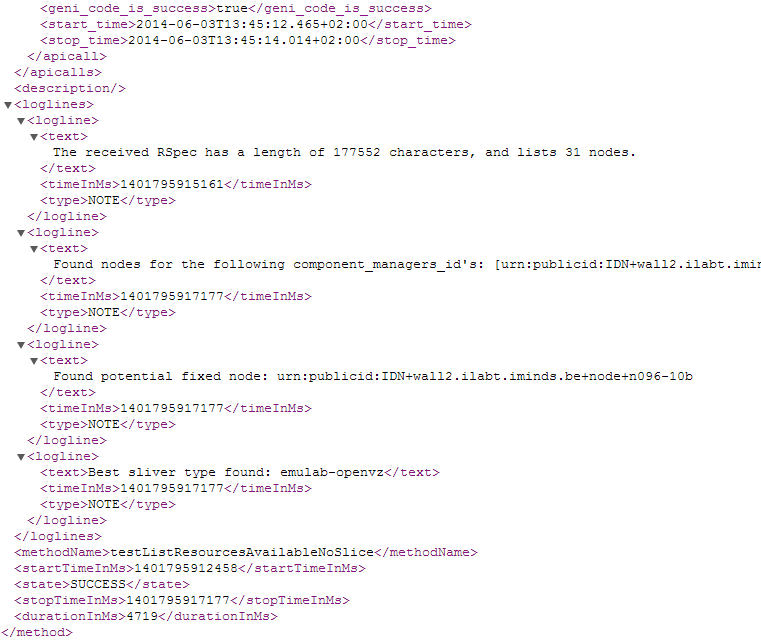
\includegraphics[width=.9\textwidth]{overviewxml}
  \caption{De originele overview in XML formaat}
\end{subfigure}
\begin{subfigure}{.45\textwidth}
  \centering
  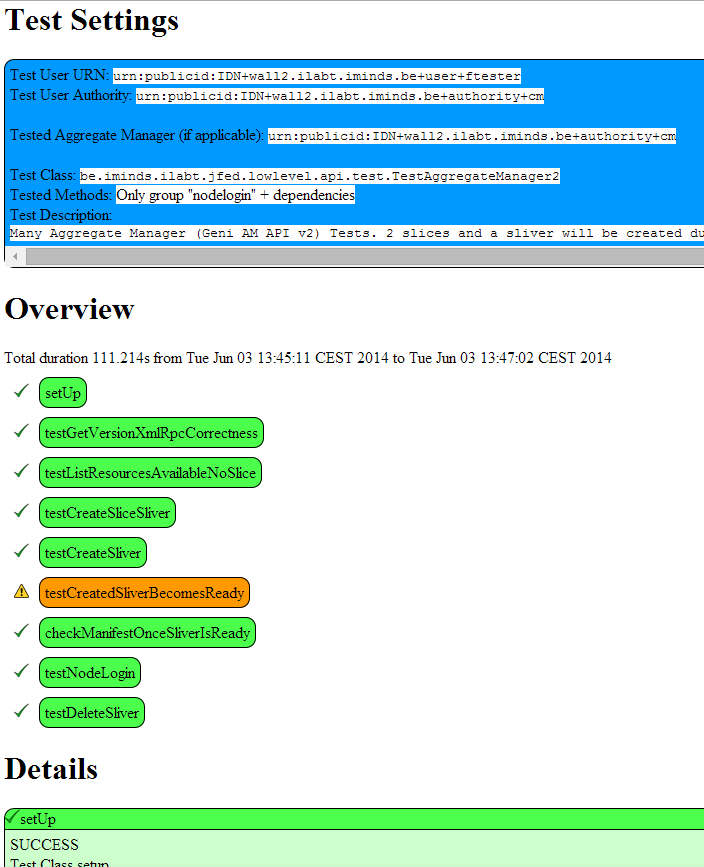
\includegraphics[width=.9\textwidth]{overviewhtml}
  \caption{Overview in html formaat}
\end{subfigure}
\caption{Naast de console uitvoer zijn ook het originele resultaat in XML formaat en het overeenkomstige HTML formaat beschikbaar.}
\end{figure}
 
\chapter{Loadtest}
{\samenvatting Deze masterproef maakt een monitoringsservice met een bijhorende monitoringsAPI. Dit systeem zal testbeds monitoren en deze data toegankelijk maken om de betrouwbaarheid van een testbed te bepalen. Naast betrouwbaarheid is echter ook de performantie van belang. Door een aantal aanpassingen aan de monitoringsservice werd tijdens de uitwerking van de masterproef ook een tool gemaakt die loadtesten kan uitvoeren. Een loadtest is een test waarbij een bestaande testen binnen een kort tijdsinterval meerdere malen uitgevoerd wordt. De loadtest zal eerst een bestaande test ophalen en deze vervolgens op meerdere threads tegelijk starten.}
\section{Doel}
\npar
Een loadtest wordt gebruikt om te kijken welke belasting een testbed kan afhandelen. Een voorbeeld van een situatie waar dit nodig is, is wanneer een leerkracht met een groep studenten het testbed wil gebruiken voor een labo. Hierbij zouden 50 studenten elk 2 computers gebruiken om tcp-congestie te testen. TCP-congestie wordt gebruikt om fileproblemen die ontstaan door het overlopen van buffers te verhelpen. Deze problemen ontstaan nadat een host meer informatie doorstuurt dan een tussenliggende router kan afhandelen. Hierdoor zal de buffer van de router overlopen, wat leidt tot verlies van pakketten. Aangezien het TCP protocol garandeert dat een overdracht zeker en compleet is, worden deze pakketten opnieuw verzonden. Als men echter de verstuur snelheid niet verlaagd, zal dit alleen maar leiden tot meer verloren pakketten.
\clearpage
\npar
Het probleem is dat de leerkracht geen garantie heeft dat het testbed dit aankan. Hierdoor zijn vele leerkrachten weerhoudend om testbeds te gebruiken voor labo's.
Om aan te tonen dat het testbed wel een belasting van 50 studenten met elk 2 nodes aankan, wordt een stresstest uitgevoerd. Een voorbeeld van een uitgevoerde stresstest is terug te vinden in bijlage A. De bedoeling van deze stresstest is om 50 login testen tegelijkertijd uit te voeren. Deze zullen een belasting veroorzaken op het testbed die opgemeten en geanalyseerd wordt. Op basis van de resultaten kan een leerkracht met een gerust hart gebruik maken van het testbed of net aangeraden worden om de groep op te delen.
\section{Uitwerking}
\npar
De uitwerking wordt weergegeven in Figuur \ref{structLoadtest}, let op de overeenkomsten met Figuur \ref{structService}, waar de monitoringsservice wordt uitgelegd. De uitwerking van de loadtest is op een aantal stappen na, gelijk aan de uitwerking van de monitoringsservice, vermits de kern van beide gelijk is. 
\npar
Figuur \ref{structLoadtest} op volgende pagina geeft de uitwerking weer. Eerst wordt de bestaande test opgehaald. Daarna wordt een threadpool aangemaakt met de grootte n; het aantal testen dat uitgevoerd moet worden. Hierdoor kunnen alle testen tegelijkertijd uitgevoerd worden wat niet mogelijk is bij de service, vermits de grootte daar beperkt is. Vervolgens wordt elke test opgestart na een instelbaar interval. Dit interval zorgt er bijvoorbeeld voor dat de testen elkaar om de 2 seconden opvolgen.
\npar
Eenmaal een test is opgestart en uitgevoerd, wordt elk resultaat geparset en doorgegeven aan de resultuploader. Deze zal de resultaten een voor een uploaden en daarbij de uitvoeringstijd van de volgende test niet aanpassen. Dat laatste zou ertoe leiden dat volgende resultaten niet meer aanvaard worden. Merk het verschil met de monitoringsservice die hier wel een aanpassing doet van het nextrun veld, zie ook bijlage B.
\npar
Na het uitvoeren van de testen zijn de resultaten van de stresstest beschikbaar via de monitoringsAPI. Doordat er in de huidige implementatie geen onderscheid wordt gemaakt tussen resultaten van de monitoringsservice en de loadtesten wordt deze databank en API gekloond. De kloon hiervan zal vervolgens dienen om de resultaten van de loadtesten op te slaan. Samenvoegen van de monitoringresultaten met de loadtest resultaten is mogelijk, maar bleek noch een prioriteit, noch noodzakelijk te zijn.
\mijnfiguur{width=1\textwidth}{structLoadtest}{De uitwerking van de loadtesten.}
%besluit

% De appendices:
\appendix
%lijst van functies
%toevoegen testen
%\chapter{Voorbeeld loadtest}
\npar
Deze bijlag is een voorbeeld van een uitgevoerde loadtest als voorbereiding voor een practicum door de Griekse universiteit van Patras. Tijdens dit practicum zullen een 50-tal studenten elk 2 PC's gebruiken om TCP congestion testen. Hierbij zal de virtual wall of wall1 gebruikt worden als testbed. Doordat alle studenten hun experiment op zeer korte tijd van mekaar zullen starten, zal een grote belasting ontstaan op het testbed. Om te kijken of het testbed dergelijke belasting aankan, wordt een loadtest van 119 PC's uitgevoerd. Deze loadtest zal het practicum simuleren en weergeven of er problemen optreden. 
\npar
Figuur \ref{verslag119pcs} geeft een overzicht van de gebruikte computers. Deze computers zijn per twee opgedeeld in slices. Figuur \ref{verslagresources} geeft een overzicht van deze slices met bijhorende status. Op deze figuur komt een groen vak overeen met een slice die gelukt is, een rood vak daarentegen duidt op problemen.
\mijnfiguur{width=1\textwidth}{verslag119pcs}{Overzicht van de verschillende slices.}
\mijnfiguur{width=1\textwidth}{verslagresources}{Status van de slices.} 
\npar
Vermits er in Figuur \ref{verslagresources} maar een pc rood is, kan besloten worden dat het testbed dergelijke belasting kan verwerken. Figuur \ref{verslaggrafiek} hieronder geeft een grafiek van de belasting van het testbed op die dag. Uiterst rechts op de figuur zijn er 2 hoge waarden zichtbaar, deze zijn veroorzaakt door de stresstest. Doordat het testbed een dubbel aantal cores ziet dan dat er werkelijk zijn, moeten de percentages verdubbeld worden. De stresstest met 119 computers geeft bijgevolg een belasting van 80\% voor een bepaalde tijd.
\mijnfiguur{width=1\textwidth}{verslaggrafiek}{Belasting van het testbed, percentages moeten verdubbeld worden.} 
\clearpage
\npar
Vervolgens werd de test herhaald met 100 gebruikers die telkens 2 computers gebruiken. De veroorzaakte belasting is te zien in Figuur \ref{verslaggrafiek100users}. Ook hier moeten de percentages verdubbeld worden wat een belasting van 90\% geeft over een langere periode.
\mijnfiguur{width=1\textwidth}{verslaggrafiek100users}{Belasting van een testbed met 100 gebruikers} 
\npar
De test met 100 gebruikers bestaat eigenlijk uit 100 testen die tegelijk draaien. Voor elke test is bijgevolg een resultaat, dat te zien is op de monitoringsinterface\footnote{Deze monitoringsinterface is een kloon van de werkende monitoringsAPI die enkel stresstesten uitvoert.}. Figuur \ref{verslag100} geeft resultaten per test voor 100 users. Het is duidelijk dat er hier en daar problemen optreden, maar dat het overgrote deel wel slaagt.
\npar
Doordat de load veel hoger is dan wat de studenten in werkelijkheid zullen doen is de stresstest succesvol. 
\mijnfiguur{width=1\textwidth}{verslag100}{Weergave per test} 
\begin{otherlanguage}{english}
\chapter{MonitoringAPI reference}
\section{About}
This chapter will provide a detailed list of methods and functions available in the monitoringAPI. The monitoringAPI provides access to all the monitoringdata, both results and configuration. The API is available at http://f4f-mon-dev.intec.ugent.be/service/index.php , however this location is not permanent. In case the url returns 404, one should contact ibcn/iminds. Keep in mind that the API is still under developpment, so things might change.
\npar
The service supports get and post requests, both are handled in the same way unless stated otherwise. A request should use http://f4f-mon-dev.intec.ugent.be/service/index.php/ as base url e.g. http://f4f-mon-dev.intec.ugent.be/service/index.php/$<$functionname$>$?$<$arguments$>$ \footnote{Of course the $<$ and $>$ shouldn't be in the actual url.}. 

\section{Introduction}
The system contains all information about the results, testbeds, testdefinitions, testinstances and the login information of users used for testing. It is important to note that these users are used by programs and are not logins for experimenters.  
\npar
A testdefinition is a definition of the test e.g. a ping test consists of a ping command while a login test uses the Aggregate manager to log in to a testbed. The definition describes the arguments used for and results returned from a test. Each definition has its own name, the testdefinitionname and an internal testtype named testtype this type tells the monitoringsservice whether or not to use the automated tester.
\npar
The testinstance on the other hand is an instance of a testdefinition e.g. a login test on the virtual wall. Each instance has an instanceid, a name and the name of its definition.

\section{Functions}
The functions needed for experimenters are listed below. Next up is a detailed explaination of each function. The current list of functions is:
\begin{enumerate}
\item List
\item Last
\item TestDefinition
\item TestInstance
\item Testbed
\item User
\item Q (GENI datastore support, use with caution)
\item AddResult (administrators only)
\item updateNextRun (administrators only)
\end{enumerate}
\npar
The return format of each call below can be change with ?format=$<$formatname$>$. 
Other than json as default format, PrettyJson is also available. PrettyJson uses the php json pretty print parameter to outline the resulting json making it more humanfriendly.
Use it by adding format=PrettyJson to any call.

\subsection{List}
\subsubsection{What}
The list function will list monitoring results because of performance and security reasons, only the last 100 results that comply with the query will be returned. Keep in mind that this is 100 for each testinstance, testbed combination. In case more is needed, one could use from and till clausules or contact ibcn/iminds.

\clearpage

\subsubsection{Arguments}
\begin{enumerate}
\item testbed: the testbed of the corresponding result
\item testdefinitionname: the name of the testdefinition of the corresponding testbed.
\item resultid: the id of the result.
\item testname: the name of the corresponding test
\item from: search results after a given timestamp NOTE: use iso 8601 format WITH timezone.
\item till: search results before a given timestamp NOTE: use iso 8601 format WITH timezone.
\item count: the last $<$count$>$ results will be returned. Limited to 100 and default also 100. The results are counted for each combination of testbed en testdefinitionname therefor list?count=50 will return the last 50 results for each test on each testbed, so when there are 2 testbeds, 100 results will be returned in total.
\end{enumerate}
\npar
It is important to note here that using from/till arguments in combination with count is not possible. Doing so will return a http 400 (bad request) error.
\subsubsection{Examples}
\begin{lt}
list?from=2014-03-18T19:29:00\&till=2014-03-19T18:29:00\&testdefinitionname=ping
&testbed=wall2
\end{lt}
Will return all the results of each\footnote{Although generally not recommended, it is possible to have multiple tests of the same type on one testbed.} pingtest on wall2 between 18/03/2014 18:29:00 and 19/03/2014 18:29:00.
\npar
\begin{lt}
list?testdefinitionname=stitch\&count=5\&testbed=wall2
\end{lt}
Will return results of the last 5 stitching tests for wall2.

\clearpage

\subsection{Last}
\subsubsection{What}
Last has the same functionality as list, but uses default count=1. It is a shortcut to get the last results of each test on each testbed.
\subsubsection{Arguments}
\begin{enumerate}
\item testbed: the testbed of the corresponding result
\item testdefinitionname: the name of the testdefinition of the corresponding testbed.
\item resultid: the id of the result.
\item testname: the name of the corresponding test
\item count: the last $<$count$>$ results will be returned. Limited to 100 and default also 100. The results are counted for each combination of testbed en testdefinitionname therefor list?count=50 will return the last 50 results for each test on each testbed, so when there are 2 testbeds, 100 results will be returned in total.
\end{enumerate}
\npar
Since last uses a default count, it is not possible to use from/till arguments here. Doing so will return a http 400 (bad request) error.
\subsubsection{Examples}
\begin{lt}
last?testdefinitionname=ping
\end{lt}
Will return the last result of each\footnote{Although generally not recommended, it is possible to have multiple tests of the same type on one testbed.} pingtest of each testbed.
\npar
\begin{lt}
last?testdefinitionname=stitch\&count=5\&testbed=wall2
\end{lt}
Will return results of the last 5 stitching tests for wall2. Note that this is also possible with list.
\npar
\begin{lt}
last
\end{lt}
Returns the last result of each test on each testbed.
\clearpage
\subsection{TestDefinition}
\subsubsection{What}
This call will return the testdefinitions. A testdefinition is used to define a test.
\subsubsection{Arguments}
\begin{enumerate}
\item testdefinitionname: the name of the testdefinition.
\item testtype: the internal testtype used to determine if the test uses the automated tester or a bash command. It is not recommended for experimenters to use this.
\end{enumerate}
\subsubsection{Examples}
\begin{lt}
testdefinition?testdefinitionname=ping
\end{lt}
Will return the definition of a ping test.
\\
\subsection{TestInstance}
\subsubsection{What}
This call will return the testinstance. A testinstance is an instance of the definition; the instance will define a pingtest on a certain testbed while a definition will define that a pingtest consists of a ping command. 
\subsubsection{Arguments}
\begin{enumerate}
\item testbed: the testbed used by the test
\item testdefinitionname: the name of the testdefinition.
\item testname: name of the test.
\item testinstanceid: the id of the testinstance.
\item nextrun: field used to determine the next execution of a test. formatted in iso 8601 WITH timestamps.
\end{enumerate}
\clearpage
\subsubsection{Examples}
\begin{lt}
testinstance?testdefinitionname=stitch\&testbed=wall2
\end{lt}
Will return all the instances of the stitching type on wall2.
\begin{lt}
testinstance?nextrun=2014-06-19T12:00:00
\end{lt}
Will return all tests with nextrun $>=$ 19/06/2014 12:00:00; used by the monitoringsservice.\\

\subsection{Testbed}
\subsubsection{What}
This call will return the testbeds.
\subsubsection{Arguments}
\begin{enumerate}
\item testbedname: name of the testbed.
\item urn: urn of the testbed.
\item url: url of the testbed.
\end{enumerate}
\subsubsection{Examples}
\begin{lt}
testbed?urn=urn:publicid:IDN+wall1.ilabt.iminds.be+authority+cm
\end{lt}
Will return the information of the testbed with urn = \\
urn:publicid:IDN+wall1.ilabt.iminds.be+authority+cm (wall1).
\\
\subsection{User}
\subsubsection{What}
This call will return information about an user. Note that only users used by the monitoringservice are stored here making it impossible to see information about all users on the testbed.
\subsubsection{Arguments}
\begin{enumerate}
\item username: the name of the users.
\item userauthorityurn: the urn of the user used for authentication.
\end{enumerate}
\subsubsection{Examples}
\begin{lt}
user/username=ftester
\end{lt}
Will return the information for the ftester user.
\\
\subsection{Q}
\subsubsection{What}
This function is not real function but an argument of the list function. It is used to make this monitoringAPI compatible with the GENI datastore. However since both GENI and this API are in developpment, not every function is yet available.
\subsubsection{Arguments}
The arguments here are encoded as a json string, for more information i refer to http://groups.geni.net/geni/wiki/OperationalMonitoring and http://groups.geni.net/geni/wiki/OperationalMonitoring/DatastorePolling.
\npar
Not all of these functions are supported only these:
\begin{enumerate}
\item aggragate: it is possible to filter on aggregate name.
\item eventType: the evenname as defined by genidatastore. 
\item ts: unix timestamp in micro( 1/1000000) seconds.
\begin{enumerate}
\item gte: similar with from
\item lt: similar with till
\end{enumerate}
\end{enumerate}
\subsubsection{Example}
\begin{lt}
list?q={
  filters:{
    eventType:[ops_monitoring:is_available],
    obj:{type:aggregate,id:[wall2,wall1]}
  }
}
\end{lt}
Will return results of the is\textunderscore available\footnote{The is\textunderscore available is the GENI name for a getVersion call, so this call will return whether or not the getVersion test succeeded} test for wall1 and wall2.
\clearpage
\end{otherlanguage}

\chapter{Onderhoud, beheer en gebruik}
{\samenvatting Dit hoofdstuk richt zich tot de systeem beheerder en bespreekt hoe het onderhoud van de de monitoringsAPI en service verloopt. Hierbij wordt de nadruk gelegd op het toevoegen, verwijderen, activeren en deactiveren van testen.}
\npar
\section{Over}
\npar
Een testinstantie maakt de link tussen een testdefinitie en zijn set parameters. In volgende tekst wordt, tenzij anders vermeld, met test ook altijd een testinstantie bedoeld. Een test heeft altijd een type, dit type wordt gedefinieerd door de testdefinition die ook opgeslagen zit in de databank. De bedoeling is dat een systeembeheerder eenvoudig nieuwe testtypes kan ondersteunen door nieuwe definities aan te maken. Dit kan op meerdere manier en is hieronder beschreven.
\npar
Daarnaast heeft een test ook een nextrun veld, dit veld bevat een iso 8601 timestamp met tijdzone en geeft aan wanneer de test de volgende keer uitgevoerd moet worden. De test zal uitgevoerd worden op het moment dat de monitoringsservice (die periodiek opgestart wordt via cron) de API pollt naar testen die uitgevoerd moeten worden. Als nextrun dan in het verleden ligt, zal de test doorgestuurd worden en uitgevoerd worden. De nextrun zal aangepast worden door de monitoringsservice als volgt: $nextrun_{new} = starttime + frequency$.
\npar
Het is ook mogelijk om testen te deactiveren door het veld enabled op false te zetten. Deze testen zullen bijgevolg niet uitgevoerd worden ongeacht de waarde van hun nextrun veld. Vanzelfsprekend moet dit veld terug op true gezet worden om de test terug te activeren.

\section{Toevoegen van testen (testinstancies)}
\npar
Voor het toevoegen van een testinstanties moet er eerst gekeken worden naar het de bijhorende definitie. De definitie kan opgevraagd worden via /testdefinition?testdefinitionname=$<$definitienaam$>$ (zie ook bijlage B). Vervolgens moeten alle parameters ingesteld worden. 
\npar 
Een voorbeeld, de definitie van een list resource test is:
\begin{lt}
    "listResources": {
        "testdefinitionname": "listResources",
        "testtype": "listResources",
        "testcommand": "",
        "parameters": {
            "user": {
                "type": "user",
                "description": "user for authentication"
            },"testbed": {
                "type": "testbed",
                "description": "testbed to get the list recources from"
            },"context-file": {
                "type": "file",
                "description": "username = \n    passwordFilename = \n    pemKeyAndCertFilename = \n    userAuthorityUrn = "
            }
        },"returnValues": {
            "count": {
                "type": "int",
                "description": "free resources"
            },"rspec": {
                "type": "file",
                "description": "path of rspec file"
            }
        }
    }
\end{lt}
\npar 
Hier kan uit afgeleid worden dat een listResource test een user, testbed en context file nodig heeft om een count en rspec terug te geven. Parameters worden dan bijvoorbeeld met een python script ingevuld, zoals in het voorbeeld hieronder waarbij een listResources test voor wall2 gemaakt wordt.
\clearpage
%\begin{lt}
\begin{lstlisting}[language=Python]
import psycopg2 #postgresql databanken

#queries eerste geeft de testinstance id terug
addTestQ = "INSERT INTO testinstances (\
	testname,\
	testDefinitionName,\
	frequency,\
	nextrun,\
	enabled\
) VALUES(%s,%s,%s,%s,%s) RETURNING testinstanceid"

addParQ  = "INSERT INTO parameterInstances (\
	testinstanceId,\
	parameterName,\
	parametervalue\
) VALUES (%s,%s,%s)"

#connectie maken
con = psycopg2.connect(database=dbname,user=user,password=pass,host=durl) 
#vul overeenkomstige waarden in
cur = con.cursor()

#maak test
cur.execute(addTestQ,(\
	"wall2list,\
	"listResources",\
	3600,\
	"2014-6-1T12:00:00+00",\
	"t")\
)
testinstanceid = cur.fetchone()[0] #ophalen id

#parameters
cur.execute(addParQ,(testinstanceid,"testbed",wall2))	
cur.execute(addParQ,(testinstanceid,"user",ftester))

con.commit() #commit
\end{lstlisting}
%\end{lt}
\npar
Hiervoor moet het testbed wall2,de user ftester en de testdefinitie voor listResources bestaan.

\clearpage
\section{Toevoegen van types/definities (testdefinitions)}
\npar
Definities kunnen op meerdere manieren toegevoegd worden.
\begin{enumerate}
\item nieuw intern type
\item testdefinitie toevoegen in de databank.
\end{enumerate}

\subsection{Nieuw intern type}
Het is zo dat elke test een intern type heeft dit type komt overeen met een klasse in de monitor.testCalls package . Er wordt gebruik gemaakt van overerving waarbij er 2 groepen testen zijn: de bashtesten die een bash commando uitvoeren en de jfed automated testen die gebruik maken van de jfed automated tester. Voor de eerste groep is het aangeraden over te ervan van BashTestCall, voor de tweede groep is javaMainTestCall de klasse. Overerven is sterk aangeraden vermits deze code bevat voor het parsen van parameters en het aanroepen van de jfed automated tester. In deze overgeërfde klasse kunnen parameters vervolgens hardgecodeerd worden, bijgevolg moeten ze niet meer opgeslagen worden in de databank.
\npar
Op deze manier is het mogelijk om bijvoorbeeld een eenvoudige stitching test te maken met een aantal standaard waarden. Naast deze test zou er nog een advanced stitching test kunnen zijn waar de parameters wel opgegeven moeten worden. Beide testen zouden vervolgens verschillend in naam. Bijgevolg kan men eenvoudig kiezen tussen beide varianten door het overeenkomstige testtype te kiezen.
\npar
Merk op dat voor het gebruik van nieuwe parameter types er mogelijk aanpassingen gedaan moeten worden in de javaMainTestCall klasse. Daarnaast moet er ook een nieuwe casse toegevoegd worden bij de makeTest van de TestCallFactory.
\clearpage
\npar
Een voorbeeld voor een login test (amv2) is volgende interne klasse:
\begin{lstlisting}[language=Java]
public class LoginTestCall extends JavaMainTestCall {	
	...
    @Override
    protected ArrayList<String> getParameters(String parsedCommand) {
        ArrayList<String> commands = super.getParameters(parsedCommand);
        commands.add("--test-class");
        commands.add(
        	"be.iminds.ilabt.jfed.lowlevel.api.test.TestAggregateManager2"
        );
        commands.add("--group");
        commands.add("nodelogin");
        commands.add("--output-dir");
        commands.add(makeTestOutputDir());
        
        return commands;
    }
    ...
}
\end{lstlisting}
\npar
Merk op hoe de parameters hier hardgecodeerd worden, bijgevolg moeten deze parameters niet meer opgegeven worden bij het toevoegen van de test. Zo is hieronder een voorbeeld van python code die een instantie van bovenstaande test toevoegd, waarbij enkel een testbed en een user opgegeven moet worden. Andere parameters voor de automated tester zoals de test-class en group zijn hier niet meer nodig.
\begin{lstlisting}[language=Python]
cur.execute(addTestQ,("wall2login2","login2",loginFreq,nextRun,enabled))
testinstanceid = cur.fetchone()[0]
cur.execute(addParQ,(testinstanceid,"testbed",map['testbedname']))	
cur.execute(addParQ,(testinstanceid,"user",map['username']))
\end{lstlisting}
\npar
Merk wel op dat er ook nog altijd een definitie voor login2 aanwezig is in de databank, maar deze definitie zal de hardgecodeerde parameters niet meer bevatten. Het is echter wel noodzakelijk dat deze definitie aanwezig is, vermits zo o.a. gebruikt wordt om te kijken of alle tussen resultaten gegeven zijn wanneer er een nieuw resultaat toegevoegd moet worden.

\clearpage
\subsection{Testdefinitie toevoegen in de databank}
\npar
Een tweede manier is het toevoegen van een definitie in de databank, deze test heeft dan als intern type ofwel bash ofwel automatedTester. Bij de eerste wordt de commando tekst beschouwd als het commando, bij de tweede zijn dit de parameters die meegegeven worden aan de automated tester. Waarden van parameters kunnen opgevraagd worden door de parameter naam tussen $<$ en $>$ te plaatsen\footnote{Dit is overal zo, alle waarden tussen $<$ en $>$ zullen geparset worden en opgezocht worden bij de parameters, indien het om een parameter met type testbed en naam testbed gaat geeft $<$testbed.urn$>$ de urn van het testbed terug.}.
\npar 
Op deze manier kan het voorgaande script omgezet worden naar een automatedTestCall waarbij de parameters in de databank opgeslagen zitten. Hieronder eenvoorbeeld code in php.
\begin{lstlisting}[language=PHP]
$subQuery = "insert into parameterDefinitions (
	testDefinitionName,
	parameterName,
	parameterType,
	parameterDescription
) values ($1,$2,$3,$4);";
$query = "insert into testdefinitions(
	testDefinitionName,
	testtype,
	geniDatastoreTestname,
	geniDatastoredesc,
	geniDatastoreUnits,
	testcommand
) values($1,$2,$3,$4,$5,$6);";
\end{lstlisting}
\clearpage
\begin{lstlisting}[language=PHP]
//test toevoegen
$data = array('loginGen','automatedTester', '','','boolean', 
  '--context-file <context-file> '
. '--test-class '
. 'be.iminds.ilabt.jfed.lowlevel.api.test.TestAggregateManager2 '
. '--group nodelogin '
. '--output-dir <output-dir> '
. '-q'
    ); 
pg_query_params($con, $query, $data);

//parameters
$data = array("loginGen", "context-file", "file", "username = ftester
    passwordFilename = " . $authDir . $passfile . "
    pemKeyAndCertFilename = " . $authDir . "cert.pem
    userAuthorityUrn = <userAuthorityUrn>
    testedAggregateManagerUrn = <testedAggregateManager.urn>");
pg_query_params($con, $subQuery, $data);
...
\end{lstlisting}
\npar
Merkt op dat de parameters hier wel in bij de defintie zichtbaar zijn. Tot slot kan vermeld worden dat $<$context-file$>$ vervangen zal worden door de parameter context-file. Vermits deze parameter van het type file is, wordt er een file aangemaakt waarvan het path terrecht komt op de plaats van de $<$context-file$>$. 

\section{Troubleshooting}
\subsection{Resultaten worden niet opgeslagen door de API}
\npar
Resultaten kunnen om een van volgende redenen geweigerd worden:
\begin{enumerate}
\item het testid bestaat niet of is onjuist
\item Niet alle tussenresultaten die in de testdefinitie gedefinieerd zijn, zijn meegegeven. 
\item nextrun ligt niet na de bestaande nextrun, dit kan ontstaan door fouten met tijdzones. Normaal gezien wordt een unix timestamp gebruikt in microseconden (1/1000 000 seconde).
\end{enumerate}
De regel is ook dat ofwel alles wordt opgeslagen ofwel niets. Er wordt gebruikt gemaakt van transacties die de integriteit van de data bewaren.
\subsection{Het programma loopt vast tijdens het uitvoeren van een zelf aangemaakte testen.}
\npar 
Controleer of alle parameternamen, opgegeven in de instance, overeenkomen met de namen van de parameters in de definitie.

% De bibliografie en de index
\backmatter

\bibliography{lc-bibliografie}

%\printindex                             % Om de index af te printen, niet bij een thesis.

\end{document}